\documentclass[10pt]{article}
\usepackage[utf8]{inputenc}
\usepackage[T1]{fontenc}
\usepackage{amsmath}
\usepackage{amsfonts}
\usepackage{amssymb}
\usepackage[version=4]{mhchem}
\usepackage{stmaryrd}
\usepackage{bbold}
\usepackage{graphicx}
\usepackage[export]{adjustbox}
\graphicspath{ {./images/} }
\usepackage{caption}
\usepackage{hyperref}
\hypersetup{colorlinks=true, linkcolor=blue, filecolor=magenta, urlcolor=cyan,}
\urlstyle{same}

\title{On the Classification of APN Functions up to Dimension Five }

\author{Marcus Brinkmann ${ }^{1}$ and Gregor Leander ${ }^{2 \star}$\\
${ }^{1}$ Ruhr-Universität Bochum, Germany\\
${ }^{2}$ University of Toulon, France}
\date{}


%New command to display footnote whose markers will always be hidden
\let\svthefootnote\thefootnote
\newcommand\blfootnotetext[1]{%
  \let\thefootnote\relax\footnote{#1}%
  \addtocounter{footnote}{-1}%
  \let\thefootnote\svthefootnote%
}

%Overriding the \footnotetext command to hide the marker if its value is `0`
\let\svfootnotetext\footnotetext
\renewcommand\footnotetext[2][?]{%
  \if\relax#1\relax%
    \ifnum\value{footnote}=0\blfootnotetext{#2}\else\svfootnotetext{#2}\fi%
  \else%
    \if?#1\ifnum\value{footnote}=0\blfootnotetext{#2}\else\svfootnotetext{#2}\fi%
    \else\svfootnotetext[#1]{#2}\fi%
  \fi
}

\DeclareUnicodeCharacter{21D2}{\ifmmode\Rightarrow\else{$\Rightarrow$}\fi}
\DeclareUnicodeCharacter{27F8}{\ifmmode\Longleftarrow\else{$\Longleftarrow$}\fi}

\begin{document}
\maketitle
\captionsetup{singlelinecheck=false}


\begin{abstract}
We classify the APN functions in dimension 4 and 5 up to affine and CCZ equivalence using backtrack programming and give a partial model for the complexity of such a search. In particular, we demonstrate that up to dimension 5 any APN function is CCZ equivalent to a power function, while it is well known that in dimension 4 and 5 there exist APN functions which are not extended affine equivalent to any power function. We further calculate the total number of APN functions up to dimension 5 and present a new CCZ equivalence class of APN functions in dimension 6 .
\end{abstract}

\section*{1 Introduction}
In this paper we deal with binary almost perfect nonlinear (APN) functions. A function $s: \mathbb{F}_{2}^{n} \rightarrow \mathbb{F}_{2}^{n}$ is APN if for every non-zero $c \in \mathbb{F}_{2}^{n}$ and every $a \in \mathbb{F}_{2}^{n}$ the equation $s(x)+s(x+c)=a$ has at most two solutions. APN functions play a central role in providing resistance against differential attacks on block ciphers. They were introduced by Nyberg [1] and have since been studied extensively.

The APN property is invariant under affine transformations: Let $\alpha, \beta: \mathbb{F}_{2}^{n} \rightarrow \mathbb{F}_{2}^{n}$ be affine bijections and $\gamma: \mathbb{F}_{2}^{n} \rightarrow \mathbb{F}_{2}^{n}$ be any affine function, then with


\begin{equation*}
t=\alpha \circ s \circ \beta+\gamma \tag{1}
\end{equation*}


the function $t$ is APN if and only if $s$ is APN, and $t$ is said to be extended affine (EA) equivalent to $s$. If $\gamma \equiv 0, t$ is said to be affine equivalent to $s$ and $t$ is a bijection if and only if $s$ is. Also, if $s$ is an APN bijection, the inverse $s^{-1}$ is APN.

In [2], a more general equivalence relation was introduced that includes EA equivalence as a special case. Let $\mathcal{G}(s):=\left\{(x, s(x)) \mid x \in \mathbb{F}_{2}^{n}\right\} \subseteq \mathbb{F}_{2}^{n} \times \mathbb{F}_{2}^{n}$ be the graph of the function $s$. Then a function $t$ is $C C Z$ equivalent to $s$ if $\mathcal{G}(t)$ is affine equivalent to $\mathcal{G}(s)$ in $\mathbb{F}_{2}^{n} \times \mathbb{F}_{2}^{n}$, that is if there exists an affine bijection $\lambda \in \mathbb{F}_{2}^{2 n}$ such that $\mathcal{G}(t)=\lambda(\mathcal{G}(s))$. Note that in this case $\lambda \equiv\left(\lambda_{1}, \lambda_{2}\right)$ for two affine functions $\lambda_{1}, \lambda_{2}$ from $\mathbb{F}_{2}^{2 n}$ to $\mathbb{F}_{2}^{n}$ where $\lambda_{1}(x, s(x))$ is a bijection. It was proven in [2] that this equivalence relation stabilises the APN property.

Until recently, all known APN functions happened to be equivalent to power functions on $\mathbb{F}_{2^{n}}$ and it was an open question if that was true for all APN

\footnotetext{\begin{itemize}
  \item Reseach of G. Leander sponsored by a DAAD postdoctoral fellowship.
\end{itemize}
}
functions. In [5], infinite classes of APN functions were constructed that are EA inequivalent, but CCZ equivalent, to any power function. Then Edel, Kyureghyan and Pott [3] constructed a quadratic function from $\mathbb{F}_{2}^{10}$ to itself that they showed to be CCZ inequivalent to any power function, and shortly afterwards an infinite class of such functions was found [4].

This suggests that looking at power functions only reveals the tip of the iceberg of all APN functions. Therefore in this work we take the orthogonal approach: Rather than looking for infinite classes of APN functions, we exhaustively enumerate all APN functions up to affine, EA and CCZ equivalence for $n \leq 5$, thereby providing a solid factual basis for APN related research.

We accomplish this using backtrack programming with isomorph rejection, that is by subdividing the set of all functions into increasingly finer subsets which contain all functions coinciding on increasingly larger subsets of their domain, and rejecting subsets that do not contain a canonical representative of the desired equivalence class. This is possible because the APN and canonicity properties can be tested efficiently even on functions which are only locally determinate.

We demonstrate that the known classes of APN functions in [5] already contain all APN functions in dimensions 4 and 5 . For $n=4$, there are two EA equivalence classes, one of which is not EA equivalent to a power function. But all APN functions for $n=4$ are pairwise CCZ equivalent. For $n=5$, there are seven EA equivalence classes, two of which are not EA equivalent to any power function. Furthermore, all APN functions for $n=5$ are equivalent to one of three CCZ equivalence classes, each containing power functions. Thus, we show that all CCZ equivalence classes in dimension $n<6$ contain power functions, while in dimension 6 there exist APN functions not CCZ equivalent to any power function, see [6]. We also give a new example for such a function in Sect. 7.

All computations were performed on a Pentium 4 processor with 2.8 GHz . The results for $n=4$ are immediate, and the case $n=5$ takes about three weeks.

In this paper, we first introduce functions that are indeterminate on a part of their domain and use them to define backtrack programming formally (Sect. 2). We analyse 2-dimensional affine subspaces in an arbitrary subset of $\mathbb{F}_{2}^{n}$ (Sect. 8), which allows us to define and analyse a filter predicate for APN functions (Sect. 3). The main part of the paper describes how these techniques can be extended to cover affine, EA and CCZ equivalence (Sect. 4 and 5). We conclude by deriving further results, such as the total number of APN functions (Sect. 6) and the start of a classification in dimension 6 .

In the text, we identify vectors $a \in \mathbb{F}_{2}^{n}$ with binary numbers $\sum_{i} a_{i} 2^{i} \in \left[0 ; 2^{n}-1\right] \subset \mathbb{N}_{0}$. It is well known that functions from $\mathbb{F}_{2}^{n}$ to itself can be seen as polynomials on $\mathbb{F}_{2^{n}}$; the algebraic degree is EA (but not CCZ) invariant.

\section*{2 Templates and Backtrack Programming}
In this section, we define a convenient notation for functions which are not determinate on the whole domain $\mathbb{F}_{2}^{n}$. Such functions occur in the formal definition of backtrack programming and later-on in algorithms using backtrack.

Templates: Let $\widetilde{\mathbb{F}_{2}^{n}}:=\mathbb{F}_{2}^{n} \uplus\{\diamond\}$ be the set $\mathbb{F}_{2}^{n}$ extended by the indeterminate value $\diamond$. Then we call $\tilde{s}: \widetilde{\mathbb{F}_{2}^{n}} \rightarrow \widetilde{\mathbb{F}_{2}^{n}}$ a function template if $\tilde{s}(\diamond)=\diamond$. The degree $\operatorname{deg} \tilde{s}:=\# \tilde{s}^{-1}\left(\mathbb{F}_{2}^{n}\right)$ is defined as the number of determinate positions and the co-degree $\operatorname{codeg} \tilde{s}=2^{n}-\operatorname{deg} \tilde{s}$ as the number of indeterminate positions in $\mathbb{F}_{2}^{n}$. The template $\tilde{s}$ is said to be fully determinate if codeg $\tilde{s}=0$. The fully indeterminate template is $\tilde{\diamond} \equiv \diamond$ with $\operatorname{deg} \tilde{\diamond}=0$. We identify $\tilde{s}$ with the set of functions $s: \mathbb{F}_{2}^{n} \rightarrow \mathbb{F}_{2}^{n}$ that coincide with $\tilde{s}$ where it is determinate and write $s \in \tilde{s}$.

We define a one-step refinement of $\tilde{s}$ on $i$ as the template $\tilde{t}=\triangleleft_{i \mapsto \tilde{t}(i)} \tilde{s}$ that is determinate in one indeterminate position $i$ of $\tilde{s}$ and coincides with $\tilde{s}$ on all other positions, increasing the degree by one.

If there exists a number $k$ such that the set of determinate positions of $\tilde{s}$ is $[0 ; k-1]$ then we say that $\tilde{s}$ is a left-refined template, which can be written as a series of $k$ left-refinements $\tilde{s}=\nabla_{k-1 \mapsto \tilde{s}(k-1)}^{\ell} \cdots \nabla_{0 \mapsto \tilde{s}(0)}^{\ell} \tilde{\nabla}$. The set of all templates that are the result of any number of left-refinements of $\tilde{s}$ is notated by $\nabla_{*}^{\ell} \tilde{s}$.

A template $\tilde{s}_{\mathcal{A}}$ is said to be affine if it is affine on the restriction to its determinate positions that must form an affine subspace of $\mathbb{F}_{2}^{n}$. Any refinement $\tilde{t}=\diamond_{k \mapsto \tilde{t}(k)} \tilde{s}_{\mathcal{A}}$ induces a unique affine refinement $\tilde{t}_{\mathcal{A}}=\widehat{\mathcal{A}}_{k \mapsto \tilde{t}(k)} \tilde{s}_{\mathcal{A}}$ which is determinate on the affine subspace spanned by the determinate positions of $\tilde{t}$.

Backtrack Programming: Let the result $\rho$ be a predicate on $\mathcal{F}\left(\mathbb{F}_{2}^{n}, \mathbb{F}_{2}^{n}\right)$, the set of all functions from $\mathbb{F}_{2}^{n}$ to $\mathbb{F}_{2}^{n}$. Then ( $\rho, \phi$ ) is a backtrack problem [7] if the filter $\phi$ is a predicate on $\widehat{\vartheta}_{*}^{\ell} \widetilde{\Delta}$ satisfying for all $s \in \mathcal{F}\left(\mathbb{F}_{2}^{n}, \mathbb{F}_{2}^{n}\right)$ :


\begin{equation*}
\rho(s) \Longleftrightarrow\left(\phi(\tilde{s}) \text { for all } \tilde{s} \in \diamond_{*}^{\ell} \tilde{\triangleright} \text { such that } s \in \tilde{s}\right) \tag{2}
\end{equation*}


A backtrack problem induces an ordered tree of order and height $2^{n}$ in a natural way: The nodes are the left-refined templates in $\diamond_{*}^{\ell} \widetilde{\Delta}$ with the root node $\tilde{\diamond}$. The edges from $\tilde{s}$ to $\tilde{t}$ are the one-step left-refinements $\tilde{t}=\nabla_{d \mapsto \tilde{t}(d)}^{\ell} \tilde{s}$ where $d$ is the depth of node $\tilde{s}$. The result predicate $\rho$ labels all leaves of the tree with a boolean value. With (2), the filter predicate $\phi$ labels all nodes of the tree such that a path from the root to a leaf is labeled with TRUE at every node if and only if the leaf is labeled true by $\rho$.

The solution of a backtrack problem is the set of all $s \in \mathcal{F}\left(\mathbb{F}_{2}^{n}, \mathbb{F}_{2}^{n}\right)$ for which $\rho(s)=$ true. It is enumerated by a pre-order search through the tree, skipping all subtrees with a root labeled FALSE by $\phi$. Pruning these subtrees from the tree, we get the active search tree $T$. The filter $\phi$ determines the size and structure of $T$ and ultimatively the time complexity of the backtrack search [8].

In Algorithm 1 and 2, we use a stateful filter as an optimisation: Let $\Sigma$ be a set of states with FALSE $\in \Sigma$, and let $S_{\diamond} \in \Sigma$ be the initial state. A stateful filter is a function $\phi: \Sigma \times \mathbb{F}_{2}^{n} \rightarrow \Sigma$ such that with $S_{\phi}(\tilde{s}):=\phi_{\tilde{s}(\operatorname{deg} \tilde{s}-1)} \cdots \phi_{\tilde{s}(0)} S_{\tilde{\delta}}$ the induced filter $\hat{\phi}:=\left(S_{\phi}(\tilde{s}) \neq\right.$ FALSE) satisfies (2). Evaluation of a stateful filter at node $\tilde{s}$ can make use of any results obtained from the evaluation of the filter at ancestor nodes that are passed through with the state.

\section*{3 APN Functions}
The APN property is closely related to 2 -dimensional affine subspaces of $\mathbb{F}_{2}^{n}$. Let $\mathcal{A}(M), M \subseteq \mathbb{F}_{2}^{n}$ arbitrary, be the set of all 2-dimensional affine subspaces in $M$. Then it is easy to verify that $\mathcal{A}(M)$ consists of the sets $\{t, u, v, w\} \subseteq M$ of four pairwise different vectors with $t+u+v+w=0$.

The next Lemma proves a characterisation of APN functions that was proposed in [9]. We will reinterpret it as a sufficiently local condition for use in a backtrack problem (APN, $\phi_{\mathrm{APN}}$ ).

Lemma 1. Let $s \in \mathcal{F}\left(\mathbb{F}_{2}^{n}, \mathbb{F}_{2}^{n}\right)$. Then $s$ is APN if and only if for all $\{t, u, v, w\} \in \mathcal{A}\left(\mathbb{F}_{2}^{n}\right)$ it holds that $s(t)+s(u)+s(v)+s(w) \neq 0$.

Proof. " ⇒ ": Assume that $s$ is APN and $\{t, u, v, w\} \in \mathcal{A}\left(\mathbb{F}_{2}^{n}\right)$. Let $c:=t+u$, then we have $s(t)+s(t+c) \neq s(v)+s(v+c)$ because $v \neq t, v \neq u=t+c$ and $s$ is APN.\\
" ⟸ : Assume we have $x, y, c, a \in \mathbb{F}_{2}^{n}, c \neq 0$, such that $s(x)+s(x+c)= s(y)+s(y+c)=a$. Then $s(x)+s(y)+s(x+c)+s(y+c)=0$ and $x, y, x+c, y+c$ can not be pairwise different. But $c \neq 0$ so we find either $y=x$ or $y=x+c$.

The filter $\phi_{\text {APN }}$ can fail a left-refined template $\tilde{s}$ if $\tilde{s}(t)+\tilde{s}(u)+\tilde{s}(v)+\tilde{s}(w)=0$ for $\{t, u, v, w\} \in \mathcal{A}([0 ; \operatorname{deg} \tilde{s}-1])$ with $t=\operatorname{deg} \tilde{s}-1$. With the definition in Prop. 11, there are $\Delta$ ( $\operatorname{deg} \tilde{s}$ ) such 2-dimensional affine subspaces, each providing an opportunity for a conflict in the APN condition by not satisfying $\tilde{s}(t) \neq \tilde{s}(u)+\tilde{s}(v)+\tilde{s}(w)$. We will further show in Sect. 8 that this is the maximum number of opportunities for conflicts we can achieve in any template of the same degree. Of course, those inequations may not all be different, but under the hypothesis that those possible conflicts are all independent probability events, we propose the following model:

Proposition 2. The modeled probability that $\phi_{A P N}$ fails a template $\tilde{s} \in \diamond_{*}^{\ell} \widetilde{\nabla}$ is:


\begin{equation*}
P(\operatorname{deg} \tilde{s})=1-\left(\frac{2^{n}-1}{2^{n}}\right)^{\Delta(\operatorname{deg} \tilde{s})} \tag{3}
\end{equation*}


Proof. The probability that one $\Delta$ ( $\operatorname{deg} \tilde{s}$ ) independent conflicts does not occur is $\left(2^{n}-1\right) / 2^{n}$.

The expected value of actual conflicts can be measured by a method described by Knuth [8]. Figure 1 gives a comparison with the model for $n=6$. We can now appreciate how difficult it is to find APN functions: Because $\Delta(k)$ is approximately quadratic (see (22)), the probability for $\phi_{\mathrm{APN}}$ to fail a template of degree $k$ approaches certainty very quickly.

Although the product $\prod_{i=1}^{k} 2^{n}(1-P(k))$ gives an estimate for the number of nodes at depth $k$ in the active search tree, errors propagate multiplicatively, and the estimate is not usable for $k \gtrsim 2^{n-1}$. In particular, the estimated number of APN functions in the case $k=2^{n}$ is unreliable: For $n=4$ (resp. $n=5$ ), this is $10^{2}$ (resp. $10^{8}$ ) times the actual number of APN functions in that dimension.

\begin{figure}[h]
\begin{center}
  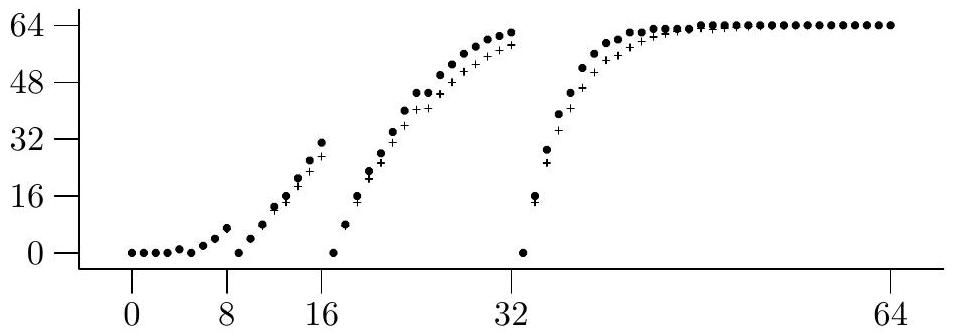
\includegraphics[alt={},max width=\textwidth]{be5710b3-fbdb-439a-8b68-1262911ccaf4-05_334_953_227_590}
\captionsetup{labelformat=empty}
\caption{Fig. 1. Actual number of conflicts for $n=6$ over depth $k$. The modeled estimates $2^{n} \cdot P(k)$ are given by crosses and the measured estimates by dots.}
\end{center}
\end{figure}

\begin{verbatim}
Algorithm 1 The stateful filter $\phi_{\mathrm{APN}}$ for APN functions with $\Sigma:=\left(\mathcal{F}\left(\mathbb{F}_{2}^{n} \backslash\right.\right.$
$\{0\} \times \mathbb{F}_{2}^{n},\{\diamond$ TRUE $\left.\left.\}\right) \times \mathcal{F}\left(\widetilde{\mathbb{F}_{2}^{n}}, \widetilde{\mathbb{F}_{2}^{n}}\right)\right) \cup\{$ FALSE $\}, S_{\tilde{\delta}}:=(\tilde{\diamond}, \tilde{\diamond})$.
    function $\phi_{\mathrm{APN}}(b,(\tilde{f}, \tilde{s}))$
        $\operatorname{var} t \leftarrow \operatorname{deg} \tilde{s} \quad \triangleright$ Depth of recursion - 1
        $\tilde{s} \leftarrow \nabla_{\operatorname{deg} \tilde{s} \mapsto b}^{\ell} \tilde{s}$
        for all $x \in[0 ; t-1]$ do
            var $c \leftarrow t \oplus x$
            $\boldsymbol{\operatorname { V a r }} a \leftarrow \tilde{s}(x) \oplus \tilde{s}(t) \quad \triangleright t=x \oplus c$
            if $\tilde{f}(c, a)=$ TRUE then return FALSE $\quad \triangleright$ Table conflict
            $\tilde{f} \leftarrow \varpi_{(c, a) \mapsto \operatorname{TRUE}} \tilde{f} \quad \triangleright$ Table update
        return $(\tilde{f}, \tilde{s})$
\end{verbatim}

Algorithm 1 implements the stateful filter $\phi_{\mathrm{APN}}$. Iterating over the 2 -dimensional affine subspaces in $\{t, u, v, w\} \in \mathcal{A}([0 ; \operatorname{deg} \tilde{s}-1])$ with $t=\operatorname{deg} \tilde{s}-1$ has quadratic time complexity in $\operatorname{deg} \tilde{s}$. Our approach has linear time complexity in $\operatorname{deg} \tilde{s}$ by trading time for space. The solved equations $\tilde{s}(t)+\tilde{s}(t+c)=a$, where $c$ is chosen such that $t+c<t$, are stored as part of the state in a table $\tilde{f}$ indexed by $(c, a) \in \mathbb{F}_{2}^{n} \times \mathbb{F}_{2}^{n}$ with values in $\{$ TRUE,$\diamond$ \} A backtrack occurs when it is attempted to set a table entry to true a second time. This approach is beneficial because a single read/store operation gives information about several potential conflicts that do not occur. We assert the correctness of Algorithm 1: If a backtrack occurs, no function in $\tilde{s}$ is APN by means of $\tilde{s}(t)+\tilde{s}(t+c)+\tilde{s}\left(t^{\prime}\right)+\tilde{s}\left(t^{\prime}+c\right)=a+a=0$, where $\left\{t^{\prime}+c, t^{\prime}, t+c, t\right\} \in \mathcal{A}([0 ; t])$ is a 2 -dimensional affine subspace. On the other hand, if a function $s$ is not APN, we have $s(t)+s(t+(t+u))=s(v)+s(v+(t+u))$ for some 2-dimensional affine subspace $A=\{t, u, v, t+u+v\}$, and a backtrack will occur at depth max $A+1$ or earlier.

\begin{table}[h]
\begin{center}
\captionsetup{labelformat=empty}
\caption{Table 1. Canonical APN permutations in $\mathcal{F}\left(\mathbb{F}_{2}^{5}, \mathbb{F}_{2}^{5}\right)$ up to to affine equivalence. The algebraic degree and equivalences to power functions are also shown.}
\begin{tabular}{|l|l|l|l|l|l|l|l|l|l|l|l|l|l|l|l|l|l|l|l|l|l|l|l|l|l|l|l|l|l|l|l|l|l|}
\hline
\# & 01 & 2 & 3 & 4 & 5 & 6 & 7 & 8 & 9 & 10 & 11 & 12 & 13 & 14 & 15 & 16 & 17 & 18 & 19 & 20 & 21 & 22 & 23 & 24 & 25 & 26 & 27 & 28 & 29 & 30 & 31 &  & Aff. \\
\hline
1 & 0 & 2 & 4 & 3 & 6 & 8 & 16 & 5 & 10 & 15 & 27 & 19 & 29 & 31 & 20 & 7 & 18 & 25 & 21 & 12 & 14 & 24 & 28 & 26 & 11 & 23 & 13 & 30 & 9 & 17 & 22 & 4 & $x^{15}$ \\
\hline
2 & 0 & 2 & 4 & 3 & 8 & 13 & 16 & 5 & 11 & 21 & 31 & 23 & 15 & 19 & 30 & 6 & 28 & 29 & 9 & 24 & 27 & 14 & 18 & 10 & 17 & 12 & 26 & 7 & 25 & 20 & 22 & 3 & $x^{11}$ \\
\hline
3 & 0 & 2 & 4 & 3 & 8 & 13 & 16 & 5 & 17 & 28 & 27 & 30 & 14 & 24 & 10 & 6 & 19 & 11 & 20 & 31 & 29 & 12 & 21 & 18 & 26 & 15 & 25 & 7 & 22 & 23 & 9 & 3 & $x^{7}$ \\
\hline
4 & 0 & 2 & 4 & 3 & 8 & 16 & 28 & 5 & 10 & 25 & 17 & 18 & 23 & 31 & 29 & 6 & 20 & 13 & 24 & 19 & 11 & 9 & 22 & 27 & 7 & 14 & 21 & 26 & 12 & 30 & 15 & 2 & $x^{3}$ \\
\hline
5 & 0 & 2 & 4 & 3 & 8 & 16 & 28 & 5 & 10 & 26 & 18 & 17 & 20 & 31 & 29 & 6 & 21 & 24 & 12 & 22 & 15 & 25 & 7 & 14 & 19 & 13 & 23 & 9 & 30 & 27 & 11 & 2 & $x^{5}$ \\
\hline
\end{tabular}
\end{center}
\end{table}

\section*{4 Affine Equivalence}
We apply the Faradžev-Read[7,10] method of isomorph rejection based on the definition of a canonical representative in each equivalence class that is extremal in that class under some order, plus an efficient canonicity test on templates.

Define a total order on the functions $s \in \mathcal{F}\left(\mathbb{F}_{2}^{n}, \mathbb{F}_{2}^{n}\right)$ by the lexicographic order of their lookup tables. We extend that to a partial order on all function templates $\tilde{s}$ by letting $\tilde{s}<\tilde{t}$ if and only if $s<t$ for all $s \in \tilde{s}$ and $t \in \tilde{t}$. In any equivalence class of $\mathcal{F}\left(\mathbb{F}_{2}^{n}, \mathbb{F}_{2}^{n}\right)$, we define the canonical element to be the lexicographically smallest in the set, and we denote the set of canonical representatives by $R_{\simeq}$.

A backtrack problem ( $\rho, \phi$ ) can be restricted to canonical representatives by using the result predicate $\rho(s) \wedge\left(s \in R_{\simeq}\right)$ and the filter $\phi \wedge \phi_{\simeq}$, where the canonicity filter $\phi_{\simeq}$ never fails templates containing canonical representatives:


\begin{equation*}
\tilde{s} \cap R_{\simeq} \neq \emptyset \quad \Longrightarrow \quad \phi_{\simeq}(\tilde{s})=\text { TRUE } \tag{4}
\end{equation*}


This is a necessary but not sufficient condition for a canonicity filter. If equivalence holds, the canonicity filter is perfect. A sufficient condition is that the canonicity filter is perfect on fully determinate templates and commonly it is considerably weakened on indeterminate templates for efficiency.

We focus first on affine equivalence of APN bijections in $\mathcal{F}\left(\mathbb{F}_{2}^{n}, \mathbb{F}_{2}^{n}\right)$. We implemented a canonicity filter $\phi_{\simeq_{\mathrm{A}}}$ for affine equivalence, generalising a technique described in [11] to indeterminate templates and to functions that may not be bijective. For our filter it holds that $\phi_{\simeq_{\mathrm{A}}}(\tilde{s})=$ FALSE if and only if there exist affine bijections $\alpha, \beta$ such that $\beta \tilde{s} \alpha<\tilde{s}$. A perfect filter would check this inequation for each function in $\tilde{s}$ separately. By making $\alpha$ and $\beta$ dependent only on $\tilde{s}$ we weaken the filter, thereby decreasing specificity but increasing efficiency.

The APN filter and affine canonicity filter tend to fail different function templates, this means that they complement each other very well. We find:

Theorem 3. There are no $A P N$ permutations in $\mathcal{F}\left(\mathbb{F}_{2}^{4}, \mathbb{F}_{2}^{4}\right)$.\\
There are $5 A P N$ permutations in $\mathcal{F}\left(\mathbb{F}_{2}^{5}, \mathbb{F}_{2}^{5}\right)$ up to affine equivalence, all of those affine equivalent to power functions, see Table 1. No. 1 is equivalent to its inverse, and no. 2 (resp. 3) is equivalent to the inverse of no. 4 (resp. 5).

For dimension 4, this was already established in [9]. For dimension 5, we have shown that no further classes of APN functions exist than those of the well-known power functions.

\begin{table}[h]
\begin{center}
\captionsetup{labelformat=empty}
\caption{Table 2. Canonical APN functions in $\mathcal{F}\left(\mathbb{F}_{2}^{4}, \mathbb{F}_{2}^{4}\right)$ up to EA equivalence. The algebraic degree, equivalences to power functions, and CCZ equivalences are also shown.}
\begin{tabular}{|c|ccccccccccccccccc|c|c|c|}
\hline
$\#$ & 0 & 1 & 2 & 3 & 4 & 5 & 6 & 7 & 8 & 9 & 10 & 11 & 12 & 13 & 14 & 15 &  & EA & CCZ \\
\hline
1 & 0 & 0 & 0 & 1 & 0 & 2 & 4 & 7 & 0 & 4 & 6 & 3 & 8 & 14 & 10 & 13 & 2 & $x^{3}$ & can. \\
2 & 0 & 0 & 0 & 1 & 0 & 2 & 4 & 7 & 0 & 4 & 6 & 3 & 8 & 14 & 11 & 12 & 3 & cf. [5] & 1 \\
\hline
\end{tabular}
\end{center}
\end{table}

We now turn to arbitrary APN functions in $\mathcal{F}\left(\mathbb{F}_{2}^{n}, \mathbb{F}_{2}^{n}\right)$ and EA equivalence. Let $B_{\mathcal{A}}:=\left\{0,2^{0}, 2^{1}, \ldots, 2^{n-1}\right\}$ be the affine standard basis of $\mathbb{F}_{2}^{n}$. Note that every function $s$ is EA equivalent to a function $t \leq s$ which vanishes on $B_{\mathcal{A}}$ by letting $t:=s+\gamma$, where $\gamma$ is affine and coincides with $s$ on $B_{\mathcal{A}}$. Thus, all EA canonical representatives vanish on $B_{\mathcal{A}}$. It also follows that $\phi_{\simeq_{\mathrm{A}}}$ satisfies (4) for an EA canonicity filter on such functions:

Proposition 4. Let the template $\tilde{s}$ vanish on its determinate positions of $B_{\mathcal{A}}$. If $\phi_{\simeq_{A}}(\tilde{s})=$ FALSE then there exist affine bijections $\alpha, \beta$ and an affine function $\gamma$ such that $\tilde{t}:=\beta \tilde{s} \alpha+\gamma$ (with $\diamond+x=\diamond$ for all $x \in \mathbb{F}_{2}^{n}$ ) vanishes on its determinate positions of $B_{\mathcal{A}}$ and $\tilde{t}<\tilde{s}$.

The filter $\phi_{\simeq_{\mathrm{A}}}$ is not perfect on the leave nodes (with regards to EA equivalence) and thus not an EA canonicity filter, but an implementation of such a filter is not efficient enough to be used in a backtrack search in small dimensions (see also Sect. 7). Thus, we used $\phi_{\simeq_{\mathrm{A}}}$ anyway, thereby finding $16(n=4)$ resp. $11768(n=5)$ candidates for EA canonical representatives, which were further analysed using the techniques described in Sect. $5 .^{3}$ We find:

Theorem 5. There are 2 APN functions in $\mathcal{F}\left(\mathbb{F}_{2}^{4}, \mathbb{F}_{2}^{4}\right)$ up to $E A$ equivalence, see Table 2. One of those is EA equivalent to a power function.

There are 7 APN functions in $\mathcal{F}\left(\mathbb{F}_{2}^{5}, \mathbb{F}_{2}^{5}\right)$ up to EA equivalence, see Table 3. Five of those are $E A$ equivalent to a power function.

Note that the three APN functions in Table 2 and 3 that are EA inequivalent to any power function actually belong to the EA equivalence classes of the infinite families of APN functions


\begin{align*}
& s(x)=x^{2^{i}+1}+\left(x^{2^{i}}+x+1\right) \operatorname{tr}\left(x^{2^{i}+1}\right) \text { for } n=4, i=1  \tag{5}\\
& s(x)=x^{2^{i}+1}+\left(x^{2^{i}}+x\right) \operatorname{tr}\left(x^{2^{i}+1}+x\right) \text { for } n=5, i=1,2 \tag{6}
\end{align*}


as given by Theorem 1 and 3 of [5]. Our contribution here is that there are no further equivalence classes with APN functions in these dimensions.

\footnotetext{${ }^{3}$ After rejecting 14 (resp. 11760) non-canonical candidates with a weak EA canonicity test, we used that the algebraic degree is an EA invariant and examined the canonicity of the remaining 2 (resp. 5) candidates by equivalence tests exploiting self-equivalences (see Note 9).
}\begin{table}[h]
\begin{center}
\captionsetup{labelformat=empty}
\caption{Table 3. Canonical APN functions in $\mathcal{F}\left(\mathbb{F}_{2}^{5}, \mathbb{F}_{2}^{5}\right)$ up to EA equivalence. The algebraic degree, equivalences to power functions, and CCZ equivalences are also shown.}
\begin{tabular}{|l|l|l|l|l|l|l|l|l|l|l|l|l|l|l|l|l|l|l|l|l|l|l|l|l|l|l|l|l|l|l|l|l|l|l|l|l|}
\hline
\# & 01 &  & 2 & 3 & 4 & 5 & 6 & 7 & 8 & 9 & 10 & 1 &  & 12 & 13 & 14 & 15 & 16 & 17 & 18 & 19 & 20 & 21 & 22 & 23 & 24 & 25 & 26 & 27 & 28 & 29 & 30 & 31 &  & EA & CCZ \\
\hline
1 & 0 & 0 & 0 & 1 & 0 & 2 & 4 & 7 & 0 & 4 & 8 &  & 13 & 16 & 22 & 28 & 27 & 0 & 8 & 16 & 25 & 5 & 15 & 17 & 26 & 22 & 26 & 14 & 3 & 3 & 13 & 31 & 16 & 2 & $x^{5}$ & can. \\
\hline
2 & 0 & 0 & 0 & 1 & 0 & 2 & 4 & 7 & 0 & 4 & 8 &  & 13 & 16 & 22 & 28 & 27 & 0 & 8 & 16 & 25 & 5 & 15 & 17 & 26 & 27 & 23 & 3 & 14 & 14 & 0 & 18 & 29 & 2 & $x^{3}$ & can. \\
\hline
3 & 0 & 0 & 0 & 1 & 0 & 2 & 4 & 7 & 0 & 4 & 8 &  & 13 & 16 & 22 & 29 & 26 & 0 & 8 & 16 & 25 & 5 & 15 & 19 & 24 & 7 & 11 & 27 & 22 & 26 & 20 & 1 & 14 & 3 & [5] & 1 \\
\hline
4 & 0 & 0 & 0 & 1 & 0 & 2 & 4 & 7 & 0 & 4 & 8 &  & 13 & 16 & 22 & 29 & 26 & 0 & 8 & 16 & 25 & 5 & 15 & 19 & 24 & 10 & 6 & 22 & 27 & 23 & 25 & 12 & 3 & 3 & [5] & 2 \\
\hline
5 & 0 & 0 & 0 & 1 & 0 & 2 & 4 & 8 & 0 & 3 & 6 &  & 12 & 7 & 16 & 25 & 23 & 0 & 7 & 3 & 22 & 28 & 19 & 9 & 0 & 19 & 8 & 15 & 28 & 21 & 9 & 29 & 2 & 4 & $x^{15}$ & can. \\
\hline
6 & 0 & 0 & 0 & 1 & 0 & 2 & 4 & 8 & 0 & 3 & 6 &  & 16 & 8 & 21 & 26 & 29 & 0 & 5 & 12 & 27 & 20 & 6 & 31 & 16 & 7 & 31 & 8 & 22 & 9 & 26 & 17 & 11 & 3 & $x^{11}$ & 2 \\
\hline
7 & 0 & 0 & 0 & 1 & 0 & 2 & 4 & 8 & 0 & 3 & 6 &  & 16 & 8 & 21 & 26 & 29 & 0 & 6 & 15 & 24 & 18 & 3 & 17 & 30 & 2 & 29 & 14 & 20 & 25 & 13 & 9 & 23 & 3 & $x^{7}$ & 1 \\
\hline
\end{tabular}
\end{center}
\end{table}

\section*{5 CCZ Equivalence}
Because CCZ equivalence requires that the graph of a function is mapped to a graph, it does not seem feasible to write an efficient filter that operates on indeterminate templates. But EA equivalence implies CCZ equivalence, so we only need to consider CCZ equivalences among EA canonical representatives, which form our new candidate sets. We used three techniques: Invariants, canonicity tests and equivalence tests.

We note that the equivalence test described below is barely efficient enough to solve the classification problem in dimension 5 . A much faster method is given in [6] by reducing CCZ equivalence to equivalence of certain extended codes, a problem for which more efficient algorithms are known. Our method is more fundamental, and has the advantage that it allows for variations such as testing for CCZ canonicity instead of equivalence, which can be useful to reduce the candidate set in greater dimensions (see Sect. 7).

We further note that Theorem 6 below can readily be derived from Theorem 5 using various results in [5] and [12]. In this section we describe a systematic approach to the classification problem, which works in principle for arbitrary (not necessarily power) APN functions in any dimension and can be transfered to other equivalence relations such as EA equivalence.\\
$C C Z$ Invariants: The extended Walsh spectrum of $s$ is the multi-set $W_{s}:= \left\{\left|w_{s}(a, b)\right| \mid a, b \in \mathbb{F}_{2}^{n}, b \neq 0\right\}$ where $w_{s}(a, b)=\sum_{x \in \mathbb{F}_{2}^{n}}(-1)^{b s(x)+a x}$, and was shown in [2] to be a CCZ invariant. For $n=4$, both candidates have the same Walsh spectrum. But for $n=5$, the candidates with degree 2 and 3 have the Walsh spectrum $(0 ; 527),(8 ; 496),(32 ; 1)$ given as (value; multiplicity), while the candidate with degree 4 has the Walsh spectrum $(0 ; 217),(4 ; 465)$, $(8 ; 310),(12 ; 31),(32 ; 1)$. Thus, the Walsh spectrum partitions the CCZ equivalence classes in dimension 5 into two sets to be treated separately.

CCZ Canonicity: Clearly the smallest EA canonical representative in each partition with different invariants is also a CCZ canonical representative. We modified Algorithm 2 below to determine CCZ canonicity of arbitrary functions $s$. The modified algorithm finds any function $t<s$ with $t \simeq_{\mathrm{CCZ}} s$ if such a function exists, otherwise it fails. This algorithm allows to quickly eliminate no. 3 and 4

\begin{verbatim}
Algorithm 2 A filter $\phi_{\pi}$ for use in a CCZ equivalence test $s \simeq_{\mathrm{CCZ}} t$.
    function $\phi_{\pi}((d, \tilde{\lambda}, \tilde{\pi}), a)$
        if $\tilde{\pi}(d) \neq \diamond$ then return $(d+1, \tilde{\lambda}, \tilde{\pi}) \quad \triangleright$ Verified previously.
        if $\tilde{\lambda}(a, s(a)) \neq \diamond$ then return FALSE $\quad \triangleright$ Position $a$ already used.
        if $(d, t(d)) \in \tilde{\lambda}\left(\mathbb{F}_{2}^{2 n}\right)$ then return FALSE $\quad \triangleright$ Ensure bijectivy of $\tilde{\lambda}$.
        if $\phi \simeq_{\pi}((d, \tilde{\pi}), a)=$ FALSE then return FALSE $\quad \triangleright$ Self-equivalences, see text.
        $\tilde{\pi} \leftarrow \diamond_{d \mapsto a} \tilde{\pi}$
        $\operatorname{var} \tilde{\lambda}^{\prime} \leftarrow \diamond_{(a, s(a)) \mapsto(d, t(d))}^{\mathcal{A}} \tilde{\lambda}$
        for all $(x, s(x)) \in \tilde{\lambda}^{\prime-1}(\mathcal{G}(t)) \backslash \tilde{\lambda}^{-1}(\mathcal{G}(t))$ do $\quad \triangleright$ Follow implications.
            $\operatorname{var}\left(y, t_{y}\right) \leftarrow \tilde{\lambda}^{\prime}(x, s(x))$
            if $\tilde{\pi}(y) \neq \diamond$ then return FALSE $\quad \triangleright$ Ensure bijectivity of $\tilde{\lambda}_{1}^{\prime}(x, s(x))$.
            if $t_{y} \neq t(y)$ then return FALSE $\quad \downarrow$ Ensure $\mathcal{G}(t) \supseteq \tilde{\lambda}^{\prime}(\mathcal{G}(s)) \backslash\{\diamond\}$.
            if $\phi \simeq_{\pi}\left((y, \tilde{\pi}), t_{y}\right)$ then return FALSE $\quad \triangleright$ Self-equivalences, see text.
            $\tilde{\pi} \leftarrow \diamond_{y \mapsto x} \tilde{\pi}$
        return $\left(d+1, \tilde{\lambda}^{\prime}, \tilde{\pi}\right)$
\end{verbatim}

in Table 3. For the other candidates in dimension 5 it is too inefficient to be of value. However, the canonicity test proved useful in dimension 6 and greater.\\
$C C Z$ Equivalence: Algorithm 2 implements an efficient test for CCZ equivalence of functions $s, t \in \mathcal{F}\left(\mathbb{F}_{2}^{n}, \mathbb{F}_{2}^{n}\right)$ using a backtrack problem ( $\rho, \phi$ ), where $\rho(\sigma)$ if and only if there exists an affine bijection $\lambda=\left(\lambda_{1}, \lambda_{2}\right)$ with $\mathcal{G}(t)=\lambda(\mathcal{G}(s))$ such that $\pi:=\lambda_{1}(x, s(x))_{\sim}^{-1} \equiv \sigma$. The state is $\tilde{\pi}$, the search depth $d$, and the affine injective ${ }^{4}$ template $\tilde{\lambda}$, with the initial state $S_{\diamond}:=(0, \tilde{\diamond}, \tilde{\diamond})$. The nodes in the search tree correspond to left-refinements for $\pi$, such that at depth $d$ it holds that $\tilde{\lambda}(\mathcal{G}(s)) \backslash\{\diamond\}=\mathcal{G}(\tilde{t} \mid\{x \mid \tilde{t}(x) \neq \diamond\})$ for a template $\tilde{t} \ni t$ which is determinate on all positions less than $d$. ${ }^{5}$ Due to affine refinements of $\tilde{\lambda}$, it may be that $\tilde{t}$ is determinate on additional positions. The algorithm recursively finds the preimage $(a, s(a)) \in \mathcal{G}(s)$ of a point $(d, t(d)) \in \mathcal{G}(t)$ with $\pi(d)=a$, while ensuring affinity and injectivity of $\tilde{\lambda}$.

We optimize further using self-equivalences: Let $\Lambda_{t}$ be the subgroup of affine bijections $\lambda_{t}$ which stabilise $\mathcal{G}(t)$. The orbit of $\lambda$ under the action of $\Lambda_{t}$ is the set of all affine functions $\lambda^{\prime}$ which map $\mathcal{G}(s)$ to $\mathcal{G}(t)$. The group $\Lambda_{t}$ induces a permutation subgroup $\Pi_{t}$ which acts on $\pi$. The orbit of $\pi$ under $\Pi_{t}$ is the set of all permutations $\pi^{\prime}$ for which a $\lambda^{\prime}$ exists with $\pi^{\prime}=\lambda_{1}^{\prime}(x, s(x))^{-1}$ and $\mathcal{G}(t)=\lambda^{\prime}(\mathcal{G}(s))$. This allows us to search only for the canonical representative in the orbit of $\pi$ by a stateful canonicity filter $\phi_{\simeq_{\pi}}$ for $\tilde{\pi}$ that is usefully defined on arbitrary (not just left-) refinements. Note that $\Pi_{t}$ can be found incrementally using Algorithm 2 and canonicity filters derived from subgroups of $\Pi_{t}$. We describe a different application of this technique in more detail when determining the EA orbits of APN functions in Sect. 6.

\footnotetext{${ }^{4}$ A template is said to be injective if it is injective on the restriction to its determinate positions.\\
${ }^{5}$ This property explains the choice to refine $\pi$ rather than $\pi^{-1}=\lambda_{1}(x, s(x))$, and allows to modify the algorithm to test for CCZ canonicity as described above.
}To complete the classification for $n=5$, we test the remaining three candidates for canonicity after ordering them lexicographically: Beginning with the smallest of the candidates, we test its CCZ equivalences against all known CCZ canonical representatives in the same partition with respect to invariants. If the candidate is not equivalent to any of those, it is itself a canonical representative and we add it to the list of known ones to test against after developing an optimized equivalence test as described above. This naive approach at isomorph rejection (cf. Sect. 4) is reasonable here because there is only a small number of such canonical representatives. In fact we find:

Theorem 6. All APN functions in $\mathcal{F}\left(\mathbb{F}_{2}^{4}, \mathbb{F}_{2}^{4}\right)$ are pairwise $C C Z$ equivalent.\\
There are only three $A P N$ functions in $\mathcal{F}\left(\mathbb{F}_{2}^{5}, \mathbb{F}_{2}^{5}\right)$ up to $C C Z$ equivalence. They are no. 1, 2, and 5 respectively in Table 3. Any APN function in $\mathcal{F}\left(\mathbb{F}_{2}^{5}, \mathbb{F}_{2}^{5}\right)$ is $C C Z$ equivalent to a power function.

\section*{6 Total Number of APN Functions}
We define $G \subset \mathcal{F}\left(\mathbb{F}_{2}^{n}, \mathbb{F}_{2}^{n}\right)^{3}$ as the set of all $(\alpha, \beta, \gamma) \in G$, where $\alpha$ is an affine bijection, $\beta$ is a linear bijection, and $\gamma$ is an affine function. We define a group structure on $G$ by:


\begin{align*}
\left(\alpha^{\prime}, \beta^{\prime}, \gamma^{\prime}\right) \cdot(\alpha, \beta, \gamma) & :=\left(\alpha \alpha^{\prime}, \beta^{\prime} \beta, \beta^{\prime} \gamma \alpha^{\prime}+\gamma^{\prime}\right)  \tag{7}\\
1_{G} & :=(i d, i d, 0) \tag{8}
\end{align*}


The group $G$ acts on $\mathcal{F}\left(\mathbb{F}_{2}^{n}, \mathbb{F}_{2}^{n}\right)$ by means of


\begin{equation*}
(\alpha, \beta, \gamma) \cdot s=\beta s \alpha+\gamma \tag{9}
\end{equation*}


and the orbit $G s$ is exactly the EA equivalence class of $s$ (the affine component of $\beta$ is subsumed by $\gamma$ ). We have $|G s|=|G| /\left|G_{s}\right|$ for the size of the EA equivalence class of $s$, where $G_{s}=\{(\alpha, \beta, \gamma) \in G \mid \beta s \alpha+\gamma=s\}$ is the stabiliser of $s$.

The order of $G$ is easy to calculate, as the number of linear permutations is well known (see sequence A002884 in [13]):


\begin{equation*}
|G|=\left|G^{\alpha}\right| \cdot\left|G^{\beta}\right| \cdot\left|G^{\gamma}\right|=\left(2^{n} \cdot \prod_{i=0}^{n-1}\left(2^{n}-2^{i}\right)\right) \cdot\left(\prod_{i=0}^{n-1}\left(2^{n}-2^{i}\right)\right) \cdot\left(2^{n}\right)^{n+1} \tag{10}
\end{equation*}


To determine the order of $G_{s}$, we first show that for the specific APN functions we are considering, it is sufficient to look at the $\alpha$ component of elements in $G_{s}$.

Lemma 7. Let $s \in \mathcal{F}\left(\mathbb{F}_{2}^{n}, \mathbb{F}_{2}^{n}\right)$ such that $s\left(\mathbb{F}_{2}^{n}\right)$ contains a linear basis and $s^{-1}(0)$ an affine basis of $\mathbb{F}_{2}^{n}$. If $(\alpha, \beta, \gamma) \in G_{s}$, then $\beta$ and $\gamma$ are uniquely determined by $\alpha$, that is, if also $\left(\alpha, \beta^{\prime}, \gamma^{\prime}\right) \in G_{s}$, then already $\beta \equiv \beta^{\prime}$ and $\gamma \equiv \gamma^{\prime}$.

Proof. We have for all $x \in \mathbb{F}_{2}^{n}$ :


\begin{equation*}
\beta(s \alpha(x))+\gamma(x)=\beta^{\prime}(s \alpha(x))+\gamma^{\prime}(x) \tag{11}
\end{equation*}


Evaluating (11) on $(s \alpha)^{-1}(0)$ gives $\gamma \equiv \gamma^{\prime}$ on an affine span of $\mathbb{F}_{2}^{n}$, and thus by affinity of $\gamma$ and $\gamma^{\prime}$ on all of $\mathbb{F}_{2}^{n}$. Canceling $\gamma$ gives $\beta \equiv \beta^{\prime}$ on the linear span that is the image of $s$, and thus by linearity of $\beta$ and $\beta^{\prime}$ on all of $\mathbb{F}_{2}^{n}$.

Corollary 8. Let $s \in \mathcal{F}\left(\mathbb{F}_{2}^{n}, \mathbb{F}_{2}^{n}\right)$ be $A P N$ and an $E A$ canonical representative. If $(\alpha, \beta, \gamma) \in G_{s}$, then $\beta$ and $\gamma$ are uniquely determined by $\alpha$.

Proof. Because $s$ is APN, it has non-null non-linearity [14].\\
Assume that $y \in \operatorname{Span}\left(s\left(\mathbb{F}_{2}^{n}\right)\right)^{\perp}$, then the canonical inner product $\langle y, s(x)\rangle$ is 0 for all $x$, and thus $y=0$ because of the non-null non-linearity of $s$. It follows that the image of $s$ spans the whole of $\mathbb{F}_{2}^{n}$. Because $s$ is EA canonical, the set $s^{-1}(0)$ contains the affine standard basis $B_{\mathcal{A}}$ (see note before Prop. 4).

Thus, to calculate the order of $G_{s}$, we only need to find the subgroup $H \subset \mathcal{F}\left(\mathbb{F}_{2}^{n}, \mathbb{F}_{2}^{n}\right)$ of all $\alpha$ for which $\beta$ and $\gamma$ exist such that $(\alpha, \beta, \gamma) \in G_{s}$. Algorithm 3 constructs a canonical set of generators for $H$ iteratively: Let $H^{k}= \left\langle h_{1}, \ldots, h_{k-1}\right\rangle \subseteq H$ be the subgroup generated by $h_{1}, \ldots, h_{k-1}$ at step $k$ of the iteration. Then $H^{k}$ acts on $H$ from the left, and the orbits induce an equivalence relation on $H$ for which we can define the canonical representatives minimal under lexicographical order. We define the next canonical generator as the smallest canonical representative that is not the identity:


\begin{equation*}
h_{k}:=\min H \backslash H^{k} \tag{12}
\end{equation*}


This element can be found by a backtrack search for $(\alpha, \beta, \gamma) \in G_{s}$, again generalising the technique described in [11] to non-bijective functions and to EA equivalence rather than just affine equivalence. In this backtrack search, $\tilde{\alpha}$ is affinely left-refined, while $\tilde{\beta}$ and $\tilde{\gamma}$ are affinely refined in parallel with $\tilde{\alpha}$ such that $\tilde{\beta} s \tilde{\alpha}+\tilde{\gamma}$ has the same degree as $\tilde{\alpha}$ and contains $s$.

The pre-order search and a stateless canonicity filter for $\tilde{\alpha}$ ensure (12): The filter $\phi_{s}^{k}$ fails $\tilde{\alpha}$ if it is identical to $i d$ or if there exists an element $h \in H^{k}$ for which $h \tilde{\alpha}<\tilde{\alpha}$. Thus, $h_{k} \in H \backslash H^{k}$ because otherwise with $h_{k}^{-1} \in H^{k}$ we have $h_{k}^{-1} h_{k}=i d<h_{k}$ and $h_{k}$ would be excluded by the filter. Specifically, the filter can be constructed from the generators $h_{1}, \ldots, h_{k-1}$ by examining the orbits $O_{x}^{k} x$ for $x \in \mathbb{F}_{2}^{n}$ under the action of those generators $O_{x}^{k} \subseteq H^{k}$ that stabilise all elements $y<x$. The canonicity requirement is then that $\tilde{\alpha}(x)=\min \tilde{\alpha}\left(O_{x}^{k} x\right) \backslash \diamond$ for all determinate positions $x$ of $\tilde{\alpha}$. A specific example is given in Note 9 .

Algorithm 3 terminates when the strictly monotonic inclusion chain $H^{k} \subsetneq H^{k+1}$ reaches $H$.

Given the generators $h_{1}, \ldots, h_{k}$, the order of $H$ can be calculated, for example using a computer algebra system such as Magma [15]. The orders of the stabilisers in dimension 4 are 5760 and 384 . In dimension 5 , the orders are 4960, 4960, 160, 160, 155, 155, and 155. Table 4 summarizes the results.

We conclude this section with a remark on how to use the stabiliser group to optimise arbitrary EA equivalence tests, as used in Sect. 4.

Note 9. We can exploit knowledge of the group $H$ in a backtrack search for EA equivalence of $s$ and an arbitrary function $t$. Clearly, $H$ acts from the left on the

\begin{table}[h]
\begin{center}
\captionsetup{labelformat=empty}
\caption{Table 4. Number of APN functions in $\mathcal{F}\left(\mathbb{F}_{2}^{n}, \mathbb{F}_{2}^{n}\right)$ absolute and as percentage of the total number $\left(2^{n}\right)^{2^{n}}$ of vectorial boolean functions.}
\begin{tabular}{|l|r|c|}
\hline
$n$ & \#APN & $\%$ \\
\hline
1 & 4 & 100 \\
2 & 192 & 75 \\
3 & 688128 & $\approx 4.1$ \\
4 & 18940805775360 & $\approx 1.0 \cdot 10^{-4}$ \\
5 & 110823678910407691468800 & $\approx 7.6 \cdot 10^{-24}$ \\
\hline
\end{tabular}
\end{center}
\end{table}

set of all $\alpha$ for which exist $\beta$ and $\gamma$ such that $\beta s \alpha+\gamma=t$. The orbits induce an equivalence relation, and we can define canonical representatives minimal under lexicographical order. The filter $\phi_{s}$ fails $\tilde{\alpha}$ if $h \in H$ exists for which $h \tilde{\alpha}<\tilde{\alpha}$.

As an example, consider the function $t$ that is no. 1 in Table 3. The group $H$ is generated by:


\begin{align*}
& h_{1}=(0)(1)(217252228)(316242329)\left(\begin{array}{lllll}
4 & 21 & 12 & 26 & 6
\end{array}\right)\left(\begin{array}{llllll}
5 & 20 & 13 & 27 & 7
\end{array}\right)\left(\begin{array}{l}
8 \\
15 \\
10 \\
30
\end{array} 19\right)(914113118)  \tag{13}\\
& h_{2}=(0)(1210134)(38795)(611151412)(1627202622)(1725302318)(19)(2124282931)  \tag{14}\\
& h_{3}=\left(\begin{array}{ll}
0 & 1
\end{array}\right)\left(\begin{array}{ll}
2 & 3
\end{array}\right)\left(\begin{array}{ll}
4 & 5
\end{array}\right)\left(\begin{array}{ll}
6 & 7
\end{array}\right)\left(\begin{array}{ll}
8 & 9
\end{array}\right)\left(\begin{array}{lll}
10 & 11
\end{array}\right)\left(\begin{array}{lll}
12 & 13
\end{array}\right)\left(\begin{array}{lll}
14 & 15
\end{array}\right)\left(\begin{array}{lll}
16 & 17
\end{array}\right)\left(\begin{array}{lll}
18 & 19
\end{array}\right)\left(\begin{array}{lll}
20 & 21
\end{array}\right)\left(\begin{array}{lll}
22 & 23
\end{array}\right)\left(\begin{array}{lll}
24 & 25
\end{array}\right)\left(\begin{array}{lll}
26 & 27
\end{array}\right)\left(\begin{array}{lll}
28 & 29
\end{array}\right)(3031) \tag{15}
\end{align*}


This leads to the following canonicity filter for $\tilde{\alpha}$ :

\begin{verbatim}
function $\phi_{s}((d, \tilde{\alpha}), a)$
    if ( $d=0$ and $a \neq 0$ ) or ( $d=1$ and $a \neq 1$ ) then return FALSE
    if $\tilde{\alpha}(2) \neq \diamond$ and $d=17,22,25$ or 28 and $a<\tilde{\alpha}(2)$ then return FALSE
    return TRUE
\end{verbatim}

\section*{7 Dimension 6}
The techniques described in this paper are sufficient to classify all APN functions in dimension 4 and 5 , but are not sufficient to treat greater dimensions. Nevertheless, they are applicable and can lead to partial results. As an example, we start a classification of APN functions in dimension 6.

Although we said earlier that the EA canonicity filter is not efficient enough to be used in a backtrack search for small dimensions, a weak version of it pays

\begin{verbatim}
Algorithm 3 Finding the generators $h_{1}, \ldots, h_{k}$ of $H$.
    var $h$ array[]
    var $k \leftarrow 1$
    var $H^{\prime} \leftarrow\langle i d\rangle$
    while $H^{\prime} \neq H$ do
        Determine $\phi_{s}^{k}$ based on $H^{\prime}=\left\langle h_{1}, \ldots, h_{k-1}\right\rangle$.
        $h_{k} \leftarrow \min H \backslash H^{\prime} \quad \triangleright$ Using backtrack search, see text.
        $k \leftarrow k+1$
        $H^{\prime} \leftarrow\left\langle h_{1}, \ldots, h_{k-1}\right\rangle$.
\end{verbatim}

\begin{table}[h]
\begin{center}
\captionsetup{labelformat=empty}
\caption{Table 5. The first 14 canonical APN functions in $\mathcal{F}\left(\mathbb{F}_{2}^{6}, \mathbb{F}_{2}^{6}\right)$ up to CCZ equivalence. All shown functions coincide on the first 33 positions, which are given first. The $\Gamma$-rank, the automorphism group of the corresponding extended code, and CCZ equivalence to the known APN functions are also shown.}
\begin{tabular}{|c|lllllllllllrrlllllllllllllllllllllll|}
\hline
$x$ & 0 & 1 & 2 & 3 & 4 & 5 & 6 & 7 & 8 & 9 & 10 & 11 & 12 & 13 & 14 & 15 & 16 & 17 & 18 & 19 & 20 & 21 & 22 & 23 & 24 & 25 & 26 & 27 & 28 & 29 & 30 & 31 & 32 \\
\hline
$s(x)$ & 0 & 0 & 0 & 1 & 0 & 2 & 4 & 7 & 0 & 4 & 6 & 3 & 8 & 14 & 10 & 13 & 0 & 8 & 16 & 25 & 5 & 15 & 17 & 26 & 32 & 44 & 54 & 59 & 45 & 35 & 63 & 48 & 0 \\
\hline
\end{tabular}
\end{center}
\end{table}

\begin{center}
\begin{tabular}{|l|l|l|l|l|l|l|l|l|l|l|l|l|l|l|l|l|l|l|l|l|l|l|l|l|l|l|l|l|l|l|l|}
\hline
\# & 33 & 34 & 35 & 36 & 37 & 38 & 39 & 40 & 41 & 42 & 43 & 44 & 45 & 46 & 47 & 48 & 49 & 50 & 51 & 52 & 53 & 54 & 55 & 56 & 57 & 58 & 59 & 60 & 61 & 62 & 63 \\
\hline
1 & 16 & 24 & 9 & 32 & 50 & 60 & 47 & 41 & 61 & 55 & 34 & 1 & 23 & 27 & 12 & 15 & 23 & 7 & 30 & 42 & 48 & 38 & 61 & 6 & 26 & 8 & 21 & 43 & 53 & 33 & 62 \\
\hline
2 & 16 & 24 & 9 & 37 & 55 & 57 & 42 & 5 & 17 & 27 & 14 & 40 & 62 & 50 & 37 & 3 & 27 & 11 & 18 & 35 & 57 & 47 & 52 & 38 & 58 & 40 & 53 & 14 & 16 & 4 & 27 \\
\hline
3 & 16 & 24 & 9 & 37 & 55 & 57 & 42 & 5 & 17 & 27 & 14 & 40 & 62 & 50 & 37 & 27 & 3 & 19 & 10 & 59 & 33 & 55 & 44 & 62 & 34 & 48 & 45 & 22 & 8 & 28 & 3 \\
\hline
4 & 16 & 26 & 11 & 32 & 50 & 62 & 45 & 33 & 53 & 61 & 40 & 9 & 31 & 17 & 6 & 35 & 59 & 41 & 48 & 6 & 28 & 8 & 19 & 34 & 62 & 46 & 51 & 15 & 17 & 7 & 24 \\
\hline
5 & 16 & 26 & 11 & 32 & 50 & 62 & 45 & 43 & 63 & 55 & 34 & 3 & 21 & 27 & 12 & 15 & 23 & 5 & 28 & 42 & 48 & 36 & 63 & 4 & 24 & 8 & 21 & 41 & 55 & 33 & 62 \\
\hline
6 & 16 & 26 & 11 & 33 & 51 & 63 & 44 & 51 & 39 & 47 & 58 & 26 & 12 & 2 & 21 & 39 & 63 & 45 & 52 & 3 & 25 & 13 & 22 & 52 & 40 & 56 & 37 & 24 & 6 & 16 & 15 \\
\hline
7 & 16 & 26 & 11 & 36 & 54 & 58 & 41 & 18 & 6 & 14 & 27 & 62 & 40 & 38 & 49 & 28 & 4 & 22 & 15 & 61 & 39 & 51 & 40 & 46 & 50 & 34 & 63 & 7 & 25 & 15 & 16 \\
\hline
8 & 16 & 26 & 11 & 36 & 54 & 58 & 41 & 33 & 53 & 61 & 40 & 13 & 27 & 21 & 2 & 39 & 63 & 45 & 52 & 6 & 28 & 8 & 19 & 38 & 58 & 42 & 55 & 15 & 17 & 7 & 24 \\
\hline
9 & 16 & 26 & 11 & 36 & 54 & 58 & 41 & 51 & 39 & 47 & 58 & 31 & 9 & 7 & 16 & 39 & 63 & 45 & 52 & 6 & 28 & 8 & 19 & 52 & 40 & 56 & 37 & 29 & 3 & 21 & 10 \\
\hline
10 & 16 & 26 & 11 & 46 & 60 & 48 & 35 & 27 & 15 & 7 & 18 & 61 & 43 & 37 & 50 & 25 & 1 & 19 & 10 & 50 & 40 & 60 & 39 & 34 & 62 & 46 & 51 & 1 & 31 & 9 & 22 \\
\hline
11 & 16 & 26 & 11 & 53 & 39 & 43 & 56 & 39 & 51 & 59 & 46 & 26 & 12 & 2 & 21 & 62 & 38 & 52 & 45 & 14 & 20 & 0 & 27 & 57 & 37 & 53 & 40 & 1 & 31 & 9 & 22 \\
\hline
12 & 16 & 26 & 11 & 53 & 39 & 43 & 56 & 43 & 63 & 55 & 34 & 22 & 0 & 14 & 25 & 50 & 42 & 56 & 33 & 2 & 24 & 12 & 23 & 57 & 37 & 53 & 40 & 1 & 31 & 9 & 22 \\
\hline
13 & 16 & 26 & 36 & 34 & 48 & 60 & 0 & 45 & 57 & 49 & 11 & 7 & 17 & 31 & 39 & 43 & 28 & 14 & 23 & 12 & 57 & 45 & 54 & 38 & 21 & 5 & 24 & 9 & 56 & 46 & 49 \\
\hline
14 & 16 & 32 & 49 & 61 & 47 & 25 & 10 & 27 & 15 & 61 & 40 & 46 & 56 & 12 & 27 & 62 & 38 & 14 & 23 & 6 & 28 & 50 & 41 & 5 & 25 & 51 & 46 & 53 & 43 & 7 & 24 \\
\hline
\multicolumn{32}{|c|}{(More CCZ equivalence classes may exist.)} \\
\hline
\end{tabular}
\end{center}

\begin{center}
\begin{tabular}{|l|l|l|l|l|l|l|l|l|l|l|l|l|l|l|}
\hline
 & 1 & 2 & 3 & 4 & 5 & 6 & 7 & 8 & 9 & 10 & 11 & 12 & 13 & 14 \\
\hline
$\Gamma$-rank & 1172 & 1146 & 1102 & 1168 & 1170 & 1170 & 1170 & 1172 & 1174 & 1166 & 1170 & 1166 & 1300 & 1158 \\
\hline
$|\operatorname{Aut}(\mathcal{C}(s))|$ & $2^{6}$ & $2^{6} 3^{2} 7$ & $2^{7} 3^{3} 7$ & $2^{6}$ & $2^{6}$ & $2^{6}$ & $2^{6}$ & $2^{6}$ & $2^{6}$ & $2^{7} 7$ & $2^{6} 5$ & $2^{6} 7$ & $2^{3}$ & $2^{6} 5$ \\
\hline
CCZ eq. & 11 [6] & 2 [6] & $x^{3}$ & 6 [6] & 8 [6] & 10 [6] & 9 [6] & 12 [6] & 13 [6] & 5 [6] & 7 [6] & 4 [6] & new & 3 [6] \\
\hline
\end{tabular}
\end{center}

off in greater dimensions. The weak EA canonicity filter fails $\tilde{s}$ if no $\alpha, \beta, \gamma$ can be found in a short time such that $\beta \tilde{s} \alpha+\gamma<\gamma$. This filter can be strengthened again by running it several times with different choices for the initial guess $\alpha(0)$, thereby adding a limited breadth-first search stragey to the mix.

We searched for lexicographically small functions in dimension 6 using this weak EA canonicity filter in addition to the affine canonicity filter. The resulting candidates were tested for CCZ canonicity as described in Sect. 5, using equivalence of the extended codes as equivalence test [6]. We found canonical representatives of 14 CCZ equivalence classes, given in Table 5. This list includes the class containing the APN power functions and the classes listed in [6]. It also contains a new CCZ equivalence class that was previously unknown.

All these classes contain quadratic functions. We also took samples from other parts of the search space, but no more CCZ equivalence classes were found this way. However, it must be said that we only examined a tiny fraction of the active search tree.

\section*{8 Affine Subspaces in $\mathbb{F}_{2}^{n}$ of Dimension 2}
The total number of 2 -dimensional affine subspaces $\# \mathcal{A}\left(\mathbb{F}_{2}^{n}\right)$ can be calculated directly or by using gaussian binomials ${ }^{6}$ and is $\binom{2^{n}}{3} / 4$. For arbitrary subsets

\footnotetext{${ }^{6}$ See also sequence A016290 in [13].
}
$M$ this is more delicate. We first calculate this number for the subsets $M= [0 ; k-1] \subseteq \mathbb{F}_{2}^{n}$ with $0 \leq k \leq 2^{n}$ and then show that this constitutes an upper bound (used in Prop. 2).

The affine hyperplanes of $\mathbb{F}_{2}^{n}$ are the sets $H_{\lambda}^{a}=\{b \mid\langle a, b\rangle=\lambda\}$ with $a \in \mathbb{F}_{2}^{n} \backslash\{0\}$ and $\lambda \in \mathbb{F}_{2}$, where $\langle$,$\rangle is the canonical inner product. The hyperplanes H_{0}^{a}$ and $H_{1}^{a}$ partition $\mathbb{F}_{2}^{n}$, which leads to the following Decomposition Lemma used in the proofs of Prop. 11 and Prop. 12:

Lemma 10. Let $M \subseteq \mathbb{F}_{2}^{n}$ and $a \in \mathbb{F}_{2}^{n} \backslash\{0\}$. Then $\mathcal{A}(M)$ can be decomposed into three disjoint subsets; with $\mathcal{A}_{+}:=\left\{A \in \mathcal{A}(M) \mid \#\left(A \cap H_{0}^{a}\right)=2\right\}$ :


\begin{equation*}
\mathcal{A}(M)=\mathcal{A}\left(M \cap H_{0}^{a}\right) \uplus \mathcal{A}\left(M \cap H_{1}^{a}\right) \uplus \mathcal{A}_{+} \tag{16}
\end{equation*}


Proof. " $\subseteq$ ": Let $A=\{t, u, v, w\} \in \mathcal{A}(M)$, then $t+u+v+w=0 \in H_{0}^{a}$. It holds that $H_{0}^{a}+H_{0}^{a}=H_{0}^{a}, H_{0}^{a}+H_{1}^{a}=H_{1}^{a}$ and $H_{1}^{a}+H_{1}^{a}=H_{0}^{a}$, so the number of elements in $A \cap H_{1}^{a}$ must be even and thus 0,2 or 4 . This means that $A$ is in $\mathcal{A}\left(M \cap H_{0}^{a}\right), \mathcal{A}_{+}$or $\mathcal{A}\left(M \cap H_{1}^{a}\right)$ respectively.

Proposition 11. Define $A(j):=\# \mathcal{A}([0 ; j-1])$ and $\Delta(0):=0, \Delta(j+1):= A(j+1)-A(j)$ with $j \in \mathbb{N}_{0}$. Let $k \in \mathbb{N}_{0}$ such that $2 \leq k \leq 2^{n}$ and $i \in \mathbb{N}_{0}$ such that $2^{i} \leq k-1<2^{i+1}$. Then the recurrence relations for $A(j)$ and $\Delta(j)$ are:


\begin{align*}
& A(k)=A\left(2^{i}\right)+A\left(k-2^{i}\right)+\binom{k-2^{i}}{2} \cdot 2^{i-1}  \tag{17}\\
& \Delta(k)=\Delta\left(k-2^{i}\right)+\left(k-2^{i}-1\right) \cdot 2^{i-1} \tag{18}
\end{align*}


Proof. We only show the relation for $\Delta(k)$ by induction over $k$, the other follows directly by $A(k)=\sum_{j=0}^{k} \Delta(j)$. Clearly $\Delta(2)=\Delta(1)+0=0$. Let now the relation be true for $j<k$. By the Decomposition Lemma 10 for $a=2^{i}$ we have:


\begin{equation*}
\mathcal{A}([0 ; k-1])=\mathcal{A}\left(\left[0 ; 2^{i}-1\right]\right) \uplus \mathcal{A}\left(\left[2^{i} ; k-1\right]\right) \uplus \mathcal{A}_{+} \tag{19}
\end{equation*}


Note that $\Delta(k)$ is the number of subspaces in $\mathcal{A}([0 ; k-1])$ which contain the point $t:=k-1$. The first term on the right hand side of (19) contributes none of those and the second term contributes $\Delta\left(k-2^{i}\right)$ by means of the bijection $j \mapsto j \oplus 2^{i}$. This leaves $\mathcal{A}_{+}$: Choose any $u \in\left[2^{i} ; k-2\right], v \in\left[0 ; 2^{i}-1\right]$, then $\{t, u, v, t+u+v\} \in \mathcal{A}_{+}$. But choosing $v^{\prime}=t+u+v$ yields the same solution, so we have to divide by 2 . On the other hand, if $\{t, u, v, w\} \in \mathcal{A}_{+}$, let without loss of generality $v, w \in H_{0}^{2^{i}}$ and thus $u \in\left[2^{i} ; k-2\right]$, because $u \in H_{1}^{2^{i}} \backslash\{t\}$.

The integer sequences $A(i)$ and $\Delta(i)$ are, starting with $i=1$ :


\begin{align*}
& A(i): \underline{0}, \underline{0}, 0, \underline{1}, 1,3,7, \underline{14}, 14,18,26,39,55,77,105, \underline{140}, \ldots  \tag{20}\\
& \Delta(i): 0,0,0,1,0,2,4,7,0,4,8,13,16,22,28,35, \ldots \tag{21}
\end{align*}


The values $A\left(2^{k}\right)$ are underlined and correspond to the number of two-dimensional affine subspaces in $\mathbb{F}_{2}^{k}$. The following equations are easy to verify and show that\\
$\Delta\left(2^{k}\right)$ is quadratic ${ }^{7}$ and $\Delta\left(2^{k}+j\right)$ is linear in $2^{k}$ for $0<j<2^{k}$.


\begin{align*}
\Delta\left(2^{k}\right) & =\frac{1}{6}\left(2^{k}-\frac{3}{2}\right)^{2}-\frac{1}{24}  \tag{22}\\
\Delta\left(2^{k}+j\right) & =\Delta(j)+\frac{1}{2}(j-1) \cdot 2^{k} \tag{23}
\end{align*}


This is analogous to the fact that the sum $\sum_{i=j}^{k+j} i$ grows linearly with $j$ but quadratic with $k$, even if the analytical treatment of the recurrence relation for $\Delta$ is more complicated. It seems the growth of $\Delta$ is well approximated by (22).

The number of affine subspaces of an arbitrary set $M \subseteq \mathbb{F}_{2}^{n}$ can be smaller than $A(\# M)$, for example it is zero if $M$ is a basis. The following proposition shows that it can never be greater. Thus, $A(\# M)$ constitutes an exact upper bound on $\# \mathcal{A}(M)$ and we establish that left-refined templates in $\diamond_{*}^{\ell} \widetilde{\text { are }}$ determinate on a domain that contains a maximum number of 2 -dimensional affine subspaces compared to other templates with the same degree.

Proposition 12. Let $M \subseteq \mathbb{F}_{2}^{n}$ be arbitrary. Then $\# \mathcal{A}(M) \leq A(\# M)$.\\
Proof. The proof is by induction over $\# M$. The claim is true for $\emptyset$ and $\{0\}$. Assume it holds for all $N \subseteq \mathbb{F}_{2}^{n}$ with $\# N<\# M$. We first demonstrate the claim for sets that are saturated (see below), and then show that every set $M$ that is not saturated can be mapped to a saturated set $M^{\prime}$ of the same size for which $\# \mathcal{A}(M) \leq \# \mathcal{A}\left(M^{\prime}\right) \leq \mathcal{A}\left(\# M^{\prime}\right)=\mathcal{A}(\# M)$.

Let $M \subseteq \mathbb{F}_{2}^{n}$ be a set. The gaps of $M$ is the set $G(M):=\mathbb{N}_{0} \backslash M$, and the minimal gap is $g:=g(M):=\min G(M) \leq 2^{n}$. The set $M$ is saturated if $M=\emptyset$, or $M=\{0\}$, or $\min G(M) \geq 2^{j}$ with $j=\left\lfloor\log _{2} \max M\right\rfloor \in \mathbb{N}_{0}$.

Assume $M \subseteq \mathbb{F}_{2}^{n}$ is saturated, $M \neq \emptyset, M \neq\{0\}$, and let $j:=\left\lfloor\log _{2} \max M\right\rfloor \in \mathbb{N}_{0}$. Then applying the Decomposition Lemma 10 for $a=2^{j}$ yields


\begin{equation*}
\# \mathcal{A}(M)=A\left(2^{j}\right)+\# \mathcal{A}\left(M \backslash\left[0 ; 2^{j}-1\right]\right)+\binom{\# M-2^{j}}{2} \cdot 2^{j-1} \leq A(\# M) \tag{24}
\end{equation*}


using $M \cap H_{0}^{2^{j}}=H_{0}^{2^{j}}$ and $\# \mathcal{A}\left(H_{0}^{2^{j}}\right)=A\left(2^{j}\right)$ for the first two terms. This leaves $\mathcal{A}_{+}$: Let $t:=\max M$. Choose any $u \in M \cap\left[2^{j} ; t-1\right], v \in\left[0 ; 2^{j}-1\right]$, then $\{t, u, v, t \oplus u \oplus v\} \in \mathcal{A}_{+}$. This gives $\left(k-2^{j}-1\right) \cdot 2^{j}$, but choosing $v^{\prime}= t \oplus u \oplus v$ yields the same solution, so we have to divide by 2 . On the other hand, if $\{t, u, v, w\} \in \mathcal{A}_{+}$, let without loss of generality $v, w \in H_{0}^{2^{j}}$ and thus $u \in M \cap\left[2^{j} ; t-2\right]$, because $u \in H_{1}^{2^{j}} \backslash\{t\}$.

Now assume $M$ is not saturated. Let $i$ be the largest integer such that $2^{i} \leq g$ if $g>0$ and let $i:=-1$ if $g=0$. Then $m:=\max M \geq 2^{i+1}$ because $M$ is not saturated, and there exists an integer $j$ with $j>i$ and $2^{j} \leq m<2^{j+1}$. Without loss of generality, assume that $g+2^{j} \in M$, else replace $M$ with its image under the affine bijection that maps $2^{j}$ to $m \oplus g$ and is invariant on all other powers of 2 , leaving $g, i$ and $j$ invariant.

\footnotetext{${ }^{7}$ See also sequence A006095 in [13].
}Define the set of sinkable elements $S:=\left\{s \in G(M) \cap H_{0}^{2^{j}} \mid s+2^{j} \in M\right\}$. We have $g \in S$. Let $\sigma$ be the permutation on $\mathbb{F}_{2}^{n}$ which swaps each element $s \in S$ with $s+2^{j}$ and does not effect any other element. It is clear that $\sigma(M)= S \uplus M \backslash\left(S+2^{j}\right)$, and thus $\# M=\# \sigma(M)$ and $g\left(M^{\prime}\right)>g(M)$.

To show that $\# \mathcal{A}(M) \leq \# \mathcal{A}(\sigma(M))$ we construct an injective mapping $s_{\mathcal{A}}: \mathcal{A}(M) \rightarrow \mathcal{A}(\sigma(M))$. By requiring that $s_{\mathcal{A}}$ leaves the values of $A \in \mathcal{A}(M)$ invariant modulo $2^{j}$, it suffices to show that $s_{\mathcal{A}}$ is injective on the subsets $\mathcal{A}_{t, u, v, w}(M):=\left\{\left\{t^{\prime}, u^{\prime}, v^{\prime}, w^{\prime}\right\} \in \mathcal{A}(M) \mid t \equiv t^{\prime}, u \equiv u^{\prime}, v \equiv v^{\prime}, w \equiv w^{\prime}\right. \left.\left(\bmod 2^{j}\right)\right\}$ with $t, u, v, w \in\left[0 ; 2^{j}-1\right]$ (not necessarily pairwise different).

To differentiate between the possible cases, we characterize a position $t<2^{j}$ by its signature, letting sig $t:=\boxminus$ if $t \notin M$ and $t+2^{j} \notin M$, sig $t:=\boxminus$ if $t \in M$ and $t+2^{j} \notin M, \operatorname{sig} t:=\boxminus$ if $t \notin M$ and $t+2^{j} \in M$ (a sinkable element), and sig $t:=\boxminus$ if $t \in M$ and $t+2^{j} \in M$. Now we can define $s_{\mathcal{A}}$ on the sets $\mathcal{A}_{t, u, v, w}$ based on the multi-set sig $\{t, u, v, w\}$.

\begin{itemize}
  \item If $S \cap\{t, u, v, w\}$ has even cardinality (i.e. 0,2 or 4 ) then let $s_{\mathcal{A}} \mid \mathcal{A}_{t, u, v, w}$ be the concatenation of all transpositions $\left(x, x+2^{j}\right)$ where $x \in S \cap\{t, u, v, w\}$.
  \item Otherwise, if $\theta \in \operatorname{sig}\{t, u, v, w\}$ then take $y:=\max \{x \in\{t, u, v, w\} \mid \operatorname{sig}(x)=\square\}$ and let $s_{\mathcal{A}} \mid \mathcal{A}_{t, u, v, w}$ be the concatenation of the transposition $\left(y, y+2^{j}\right)$ with all transpositions $\left(x, x+2^{j}\right)$ where $x \in S \cap\{t, u, v, w\}$.
  \item In all other cases the set $\mathcal{A}_{t, u, v, w}$ is actually empty, because a 2 -dimensional affine subspace in it would necessarily have an odd number of points in $H_{1}^{2^{j}}$, a contradiction.
\end{itemize}

All these restrictions of $s_{\mathcal{A}}$ are permutations generated by an even number of transpositions $\left(x, x+2^{j}\right), x \in\{t, u, v, w\}$ with $\operatorname{sig} x \in\{\mathrm{G}, \exists\}$, thereby injectively mapping the 2 -dimensional affine subspaces in $\mathcal{A}_{t, u, v, w}(M)$ to those in $\mathcal{A}_{t, u, v, w}(\sigma(M))$. Thus we have that $s_{\mathcal{A}}: \mathcal{A}(M) \rightarrow \mathcal{A}(\sigma(M))$ is well-defined and injective on its whole domain.

The minimal gap of $\sigma(M)$ is strictly greater than that of $M$, while $\max \sigma(M)$ is bounded by $2^{j+1}$. Replacing $M$ with $\sigma(M)$ and repeating the process, $\sigma(M)$ will eventually be saturated without decreasing the number of 2 -dimensional affine subspaces.

\section*{9 Acknowledgments}
We thank the reviewers for their constructive criticism which helped to improve the quality of the publication.

\section*{References}
\begin{enumerate}
  \item Nyberg, K.: Differentially uniform mappings for cryptography. In: EUROCRYPT '93. (1994) 55-64
  \item Carlet, C., Charpin, P., Zinoviev, V.: Codes, bent functions and permutations suitable for DES-like cryptosystems. Designs, Codes and Cryptography 15 (1998) 125-156
  \item Edel, Y., Kyureghyan, G., Pott, A.: A new APN function which is not equivalent to a power mapping. In: IEEE Transactions on Information Theory. Volume 52. (2006) 744-747
  \item Budaghyan, L., Carlet, C., Felke, P., Leander, G.: An infinite class of quadratic APN functions which are not equivalent to power mappings. In: IEEE International Symposium on Information Theory. (2006) 2637-2641
  \item Budaghyan, L., Carlet, C., Pott, A.: New classes of almost bent and almost perfect nonlinear polynomials. In: IEEE Transactions on Information Theory. Volume 52. (2006) 1141-1152
  \item Dillon, J.F.: APN polynomials and related codes. Banff International Research Station workshop on Polynomials over Finite Fields and Applications (Nov. 2006)
  \item Faradžev, I.A.: Constructive enumeration of combinatorial objects. In: Problèmes Combinatoires et Théorie des Graphes. Volume 260., Coloques internationaux C.N.R.S. (1978) 131-135
  \item Knuth, D.E.: Estimating the efficiency of backtrack programs. Mathematics of Computation 29 (1975) 121-136
  \item dong Hou, X.: Affinity of permutations of $\mathbb{F}_{2}^{n}$. In: Proc. of the Workshop on Coding and Cryptography. (2003) 273-280
  \item Read, R.C.: Every one a winner. Annals of Discrete Mathematics 2 (1978) 107-120
  \item Biryukov, A., Cannière, C.D., Braeken, A., Preneel, B.: A toolbox for cryptanalysis: Linear and affine equivalence algorithms. In: EUROCRYPT. (2003) 33-50
  \item Budaghyan, L., Carlet, C., Leander, G.: A class of quadratic apn binomials inequivalent to power functions. (2006)
  \item Sloane, N.J.A.: The on-line encyclopedia of integer sequences. \href{http://www}{http://www}. \href{http://research.att.com/~njas/sequences/}{research.att.com/\~{}njas/sequences/} (2007)
  \item Carlet, C. personal communication (2007)
  \item \href{http://magma.maths.usyd.edu.au/magma/}{http://magma.maths.usyd.edu.au/magma/} (2007)
\end{enumerate}

\begin{itemize}
  \item 
\end{itemize}


\end{document}